\documentclass[hidelinks,a4paper,12pt]{article}
\addtolength{\oddsidemargin}{-1.cm}
\addtolength{\textwidth}{2cm}
\addtolength{\topmargin}{-2cm}
\addtolength{\textheight}{3.5cm}
\newcommand{\HRule}{\rule{\linewidth}{0.5mm}}
\makeindex

\usepackage{longtable}
\usepackage[pdftex]{graphicx}
\usepackage{makeidx}
\usepackage{hyperref}
\hypersetup{
    colorlinks=true,
    linkcolor=black,
    filecolor=magenta,      
    urlcolor=blue,
}


% define the title
\author{Not Like This}
\title{AWS Network Visualizer Testing Document}
\begin{document}
\setlength{\parskip}{6pt}

% generates the title
\begin{titlepage}

\begin{center}
% Upper part of the page       

\includegraphics[width=1\textwidth]{./images/up-logo.jpg}\\[0.4cm]    
\textsc{\LARGE Department of Computer Science}\\[1.5cm]
\textsc{\Large COS 301 - Software Engineering}\\[0.5cm]
% Title
\HRule \\[0.4cm]

\includegraphics[width=0.05\textwidth]{./images/logo.jpg} 
{ \huge \bfseries Amazon}

\includegraphics[width=0.05\textwidth]{./images/logo.jpg}\\[0.4cm] 
{ \huge \bfseries Network Visualizer}\\[0.4cm]
{ \huge \bfseries Testing Document}\\[0.4cm]
\HRule \\[0.4cm]
% Author and supervisor
\textsc{\Large Not-Like-This}\\[0.5cm]
\begin{minipage}{0.4\textwidth}
\begin{flushleft} \large
\emph{Authors:}
\end{flushleft}
\end{minipage}
\begin{minipage}{0.4\textwidth}
\begin{flushright} \large
\emph{Student number:}
\end{flushright}
\end{minipage}

\begin{minipage}{0.4\textwidth}
\begin{flushleft} \large
Jedd {Shneier}
\end{flushleft}
\end{minipage}
\begin{minipage}{0.4\textwidth}
\begin{flushright} \large
\emph{}
u13133064
\end{flushright}
\end{minipage}

\begin{minipage}{0.4\textwidth}
\begin{flushleft} \large
Daniel {King}
\end{flushleft}
\end{minipage}
\begin{minipage}{0.4\textwidth}
\begin{flushright} \large
\emph{}
u13307607
\end{flushright}
\end{minipage}

\begin{minipage}{0.4\textwidth}
\begin{flushleft} \large
Muller {Potgieter}
\end{flushleft}
\end{minipage}
\begin{minipage}{0.4\textwidth}
\begin{flushright} \large
\emph{}
u12003672
\end{flushright}
\end{minipage}

\vfill
% Bottom of the page
{\large \today}
\end{center}
\end{titlepage}
\footnotesize
%\input{declaration_of_originality.tex}
\normalsize


\pagenumbering{roman}
\tableofcontents
\newpage
\pagenumbering{arabic}

\newpage
\section{Introduction} 
Our project is all about visualizing Amazon Web Services (AWS) virtual networks. The user can scan their entire network and in real time get a depiction of their cloud networks. It is thus a network architecture tool as well as a teaching tool for the average user to help them understand AWS network architecture and infrastructure. This project mainly focuses with performance and scalability. Scalability as very large networks connected in very complex ways need to be scanned, and performance as this needs to be done quickly and rendered in real time. These requirements reflect in our testing cases. This document details our Functional Features to be Tested, PAss/Fail Criteria, Test Deliverables,Detailed test results and finally Conclusions and Recommendations.

\subsection{Purpose}
The purpose of this document is to contain the complete suite of artifacts that describe test planning, test design, test execution, test results and conclusions drawn from the testing activity. This document holds our guidelines for testing , or results from these tests and a blueprint for future tests.


\subsection{Scope}
The scope of this document is structured as follows. The features that are considered for
testing are listed and those that have been identified from the requirements are
discussed in detail in the Unit Test Plan. Furthermore, this document outlines the test environment
and the risks involved in the testing approaches that will be followed. Assumptions and
dependencies of this test plan will also be mentioned.The Unit Test Report
discusses and concludes on the results of the tests. Finally recommendations are made for further development,issues encountered and future tests to be carried out.

\subsection{ Test Environment}



\begin{itemize}
  \item Hardware: All tests were performed on midrange laptops.4GB RAM, Intel(R)Core(TM) i5 CPU 750 @2.67 GHz
\item Software: Amazon network scanner (Back-end), Amazon network visualizer(Front-End), NetworkRESTAPI(REST Server)
\item Network: 4MB uncapped MWEB ADSL
  \item Programming Languages:Java EE (SDK-7u2),Jeresey-RX,JavaScript, Viz.js
  \item Testing Frameworks: JUnit
\item Coding Environment: InteliJ IDEA Developers edition 2016.2.1
\item Operating System: Windows 7 64 bit Professional edition
\item Internet Browsers: Firefox, Google Chrome, IE. All latest editions. 
\item Server:GlassFish Server Open Source Edition 4.1.1 
\item API: Amazon EC2 API 
\end{itemize}

\subsection{Assumptions and Dependencies}
Assumptions:
\begin{itemize}
  \item We assumed a fast, stable uncapped internet conenction.
  \item We assumed a valid user account for AWS.
\item We assumed a midrange network on the account.
\item We assumed Amazon web services would be running in all regions.
\end{itemize}
Dependencies:
\begin{itemize}
  \item Java EE installed.
  \item GlassFish installed.
\item Amazon SDK as a Maven dependency.
\item Jersey 2.16 as a Maven dependency.
\item Junit a Maven dependency.
\item Viz.js library.
\item AngularJs.
\item Bootstrap.
\end{itemize}
\newpage
\section{Unit Test Plan}

\subsection{Test Items}
The application under test is the Amazon Web Services Network Visualizer. It is divided into three separate and interconnected applications namely the Front-end(User interface and network visualizer), the Back-end(Network Scanner and Smart buffer ) and the application server(NetworkRESTServer and NetworkRESTAPI). All three are tested in their own unit tests and integration tests, and together are tested in the use case tests.
 
\subsection{Functional Features to be Tested}  
For this level of testing each of the three applications will be tested. Their individual subprograms will be tested according to their functionality and each application will be integration tested and finally perform their own unit test. The functional features to be tested in each application are as follows:

\subsubsection{Front-end}
\begin{itemize}
  \item Send data to server tested through AJAX scripts in UI HTML.
  \item Receive data from server tested through AJAX scripts in UI HTML.
  \item Visualize network jsons tested through the visualizer.js script.
  \item Iterative adding to network tested through the visualiser.js script.
  \item Dynamic menu and information box tested through the UI HTML.
  \item Button expected functionality tested through the UI HTML. 
\end{itemize}
For this unit tests will be performed with mock results from the server. The functionality of the interface will be tested through user testing.

\subsubsection{Back-end}
\begin{itemize}
  \item Connecting to AWS account tested through the Credential validation function.
  \item Scan regions tested through the AWSScanner.
  \item Threading on different levels tested through the AWSScanner.
  \item Scanning VPCS  tested through the vpcScannerThread.
   \item Scanning Subnetworks  tested through the subnetworkScannerThread.
    \item Scanning instances tested through the isntanceScannerThread.
  \item Adding scanned results to buffer tested through Sharedbuffer.
\item Constructing tree tested through Sharedbuffer.
  \item Iteratively returning the nodes as JSON objects tested through Sharedbuffer.
\end{itemize}
Unit tests are performed for each file and if they perform  expected functionality they pass. The entire Back-end will integration test and the final artifact will be tested as a whole in its own unit test.

\subsubsection{EST server}
\begin{itemize}
  \item Deploy on server tested through GlassFish.
  \item Accessible from client tested through FireFox and FireBug.
  \item Able to launch scanner with provided credentials tested through ServerAPI.
  \item Able to return on AJAX request tested through ServerAPI,FireFox and FireBug .
   \item Scanning Subnetworks  tested through the subnetworkScannerThread.
\end{itemize}
The unit tests will be done as intergration tests wit hthe first two applciations. Once the unit tests of the two applciations as a whole have been verified correct they will be used in the test of the REST server.

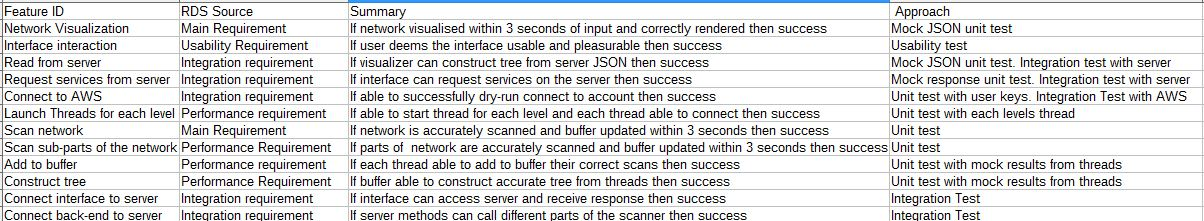
\includegraphics[width=17.3cm,height=6.5cm]{./images/table.jpg}
\newpage
 \section{Test Cases}
\subsection{Test Case 1: Login}
\subsubsection{Condition : Valid Credentials allow connection to AWS}
\subsubsection{Objective:} The purpose of this test is to test if valid users are able to connect to AWS with valid credentials.

\subsubsection{Input:}
 The following inputs will be used to test this functionality:
\begin{itemize}
  \item Valid Access Key and Secret key.
  \item Valid Access Key and invalid Secret key.
 \item Invalid Access Key and valid Secret key.
 \item Invalid Access Key and invalid Secret key.
\end{itemize}
\subsubsection{Outcome: }
The following are the expected outcomes for a pass result for the functionality:
\begin{itemize}
	\item Valid data allows for access to the AWS account in question, and invalid data is rejected by the system. 
\end{itemize}

\subsection{Test Case 2: Scan Network }
\subsubsection{Condition : Network is scanned and visualized}
\subsubsection{Objective:} The purpose of this test is to test if a full network scan and visualization is successful for a valid user.

\subsubsection{Input:}
 The following inputs will be used to test this functionality:
\begin{itemize}
  \item Click start scan.
\end{itemize}
\subsubsection{Outcome: }
The following are the expected outcomes for a pass result for the functionality:
\begin{itemize}
\item Complete network scanned and visualized on the UI.

\end{itemize}

\subsection{Test Case 3: Scan Region }
\subsubsection{Condition :Specified region  is scanned and visualized}
\subsubsection{Objective:} The purpose of this test is to test if a region scan and visualization is successful for a valid user.

\subsubsection{Input:}
 The following inputs will be used to test this functionality:
\begin{itemize}
  \item Select region to be scanned.
\end{itemize}
\subsubsection{Outcome: }
The following are the expected outcomes for a pass result for the functionality:
\begin{itemize}
\item Subtree scanned and visualized on UI.
\end{itemize}


\subsection{Test Case 4: Scan from UUID}
\subsubsection{Condition :Scan starts from specified UUID and performs scan of surrounding space}
\subsubsection{Objective:} The purpose of this test is to test if a subscan is successfully performed with a valid UUID for valid user.

\subsubsection{Input:}
 The following inputs will be used to test this functionality:
\begin{itemize}
  \item Valid vpc uuid.
  \item Valid subnetwork uuid.
 \item Valid instance uuid.
\item Invalid uuid.

\end{itemize}

\subsubsection{Outcome: }
The following are the expected outcomes for a pass result for the functionality:
\begin{itemize}
\item Subtree scanned from vpc and visualized on UI.
\item Subtree scanned from subnetwork and visualized on UI.
\item Subtree scanned from instance and visualized on UI.
\item Error message displayed.
\end{itemize}


\subsection{Test Case 5: Scan up }
\subsubsection{Condition :Scan resumes from uuid scan and scans the above region}
\subsubsection{Objective:} The purpose of this test is to test if a subscan scans up from previous scan with a valid UUID for valid user.

\subsubsection{Input:}
 The following inputs will be used to test this functionality:
\begin{itemize}
  \item Call scan on region with parents to be scanned.
   \item Call scan on region with no higher parents to be scanned.

\end{itemize}

\subsubsection{Outcome: }
The following are the expected outcomes for a pass result for the functionality:
\begin{itemize}
\item Subtree parents visualized.
\item Notification that nothing further to be scanned.

\end{itemize}

\subsection{Test Case 6: Scan Instances }
\subsubsection{Condition :Scan resumes from uuid scan and scans the below region}
\subsubsection{Objective:} The purpose of this test is to test if a subscan scans down from previous scan with a valid UUID for valid user.

\subsubsection{Input:}
 The following inputs will be used to test this functionality:
\begin{itemize}
  \item Call scan on region with sibling children to be scanned.
   \item Call scan on region with no sibling children to be scanned.

\end{itemize}

\subsubsection{Outcome: }
The following are the expected outcomes for a pass result for the functionality:
\begin{itemize}
\item Subtree  sibling children visualized.
\item Notification that nothing further to be scanned.

\end{itemize}

\subsection{Test Case 7: Get information }
\subsubsection{Condition : Information retrieved for particular node}
\subsubsection{Objective:} The purpose of this test is to test if information can be retrieved for selected nodes.

\subsubsection{Input:}
 The following inputs will be used to test this functionality:
\begin{itemize}
  \item Click on node.
  

\end{itemize}

\subsubsection{Outcome: }
The following are the expected outcomes for a pass result for the functionality:
\begin{itemize}
\item Information displayed in information box.

\end{itemize}

\subsection{Test Case 8: Get connection }
\subsubsection{Condition : Returns links of the security (and other) groups}
\subsubsection{Objective:} On call of the function the security and in some cases other groups for the node in question is returned. 

\subsubsection{Input:}
The following inputs will be used to test this functionality:
\begin{itemize}
	\item Function call with node set as parameter
	\item Function call with invalid parameters
	
	
\end{itemize}

\subsubsection{Outcome: }
The following are the expected outcomes for a pass result for the functionality:
\begin{itemize}
	\item The groups are returned.
	\item An appropriate error is handled when invalid parameters are set
	
\end{itemize}

\subsection{Test Case 9: Logout }
\subsubsection{Condition : Disconnection from the AWS account}
\subsubsection{Objective:} On click of the logout button the saved user information and the connection to the AWS account is lost. 

\subsubsection{Input:}
The following inputs will be used to test this functionality:
\begin{itemize}
	\item Logout button click.
	
	
\end{itemize}

\subsubsection{Outcome: }
The following are the expected outcomes for a pass result for the functionality:
\begin{itemize}
	\item The system is disconnected from the account.
	\item User information is lost
	
\end{itemize}

\subsection{Item Pass/Fail Criteria}

\begin{itemize}
\item Valid keys must result in connection to AWS.
\item Scan must produce a visualized scanned network that matches the AWS network.
\item Scan of region must produce the region subtree that matches the subtree visualized in full scan.
\item Scan from uuid must produce a  subtree that matches the subtree visualized in full scan.
\item Scan up must produce a subtree that matches the subtree visualized by the parent node.
\item Scan Instances must produce a subtree that matches the subtree visualized in instance.
\item The information needs to match the information for the node got through command line interface.
\item The groups in question need to be returned
\item The system is disconnected from the account, and user information is lost. 
\end{itemize}
\newpage
\section{Unit Test Report}

\subsection{Detailed Test Results}
\subsubsection{Overview of Test Results}
The individual unit tests of each part of the applciations were all successful. the applciations themselves passed their unit tests. The intergration tests did not have any failures. The first 4  test cases as well as the last test case succeded. The scan up and scan down test case failed. This is due to a bug in the construction of the network tree in the buffrer.Junit was used in unit tests with the neccesary mock objects and the actual objects were used in the integration tests. The ability to run automated repeatable tests vastly sped up our testing.
\subsubsection{Test Case 1}
Valid keys were used to connect to AWS. Invalid keys threw an exception that was caught as intended.
\subsubsection{Test Case 1 Pass}
\subsubsection{Test Case 2}
Network scanned and visualized matched what was expected.
\subsubsection{Test Case 2 Pass}
\subsubsection{Test Case 3}
Region scanned and visualized matched the subtree of the region found in the full scan.
\subsubsection{Test Case 3 Pass}
\subsubsection{Test Case 4}
Subnetwork scanned from uuid matched the subtree of the region found in the full scan.
\subsubsection{Test Case 4 Pass}
\subsubsection{Test Case 5}
Subnetwork scanned matched the subtree of the region found in the full scan.
\subsubsection{Test Case 5 Pass}
\subsubsection{Test Case 6}
Subnetwork scanned matched the subtree of the region found in the full scan.
\subsubsection{Test Case 6 Pass}
\subsubsection{Test Case 7}
Information retrieved from node click matched node output from command line.
\subsubsection{Test Case 7 Pass}
\subsubsection{Test Case 8}
The groups in question were returned
\subsubsection{Test Case 8 Pass}
\subsubsection{Test Case 9}
The system was disconnected from the account, and user information was lost.
\subsubsection{Test Case 9 Pass}

\subsection{Other}
\subsubsection{Maven}
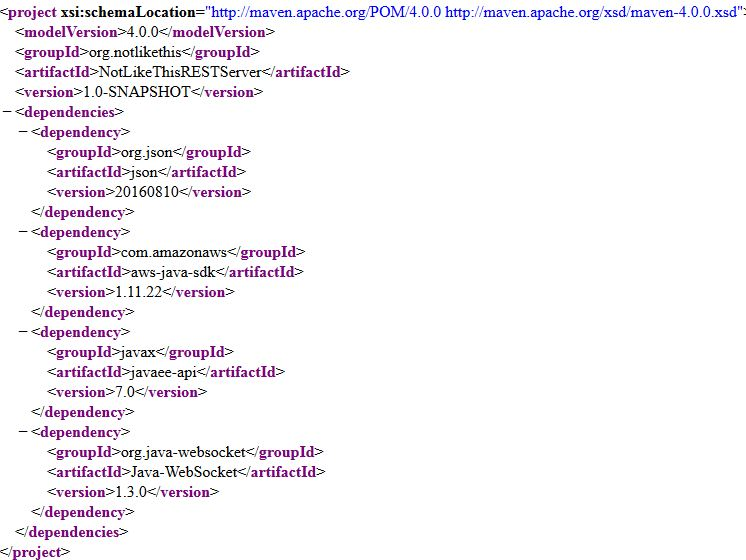
\includegraphics[width=17.3cm,height=12.5cm]{./images/maven.jpg}
\subsubsection{Contracts and Mock objects}
Our contracts for  Scanner, Buffer, NetworkTree and Subscanner allowed great flexibility  in development and in testing. Plugging in mock objects that gave expected results allowed us to confrim unit tests of the intergrated concrete parts.
\subsubsection{Application Server}
Our application is currently deployed to a GlassFish Server however our exploded WAR file can easily be deployed to a Tomcat server(Or any other application server). However the necessary maven dependencies will be required to be downloaded and the server configuration set up to deploy the artifact.

\subsection{Conclusions and Recommendations}
Our system is working as intended. However due to the intense need for performance and scalability factors the code can always be improved. In the future performance and scalability tests need be added and used continuously to fine-hone the system to a point where additional functionality can be considered and implemented. 

\end{document}
